%\chapter*{Introduction}
\chapter{Introduction}
%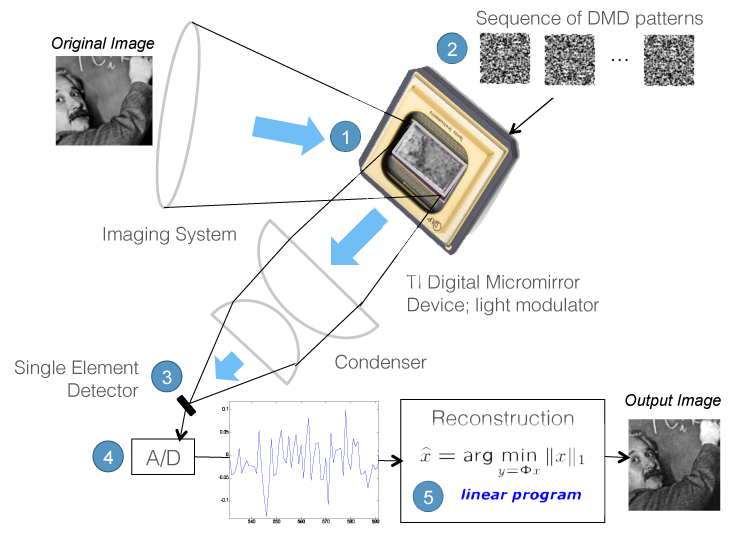
\includegraphics{Img1.png}
%\addcontentsline{toc}{chapter}{Introduction}
\section{Motivation}
Compressed sensing (CS) is a novel technique based on the discoveries done by Candes \textit{et al}. \cite{CandesR07} and Donoho \cite{Donoho01}. They showed that as long as certain conditions are met, a signal can be fully recoverd from a small number of measurements. Due to this fact, CS is suitable for many Signal Processing (SP) applications and specifically image processing. An example of this are the publications made by Duearte \textit{et al}. and Wakin \textit{et al}. \cite{duarte2008single,wakin2006architecture}. In their work they explained their ideas for architecting an imaging sensor capable of sampling and compressing the signal at the same time. Such a sensor offers the advantage of taking less samples than those needed by concentional sensors and there is no extra compression face after the measuremnts are taken, thereby saving computation worload. As a result, the indutry and the research community have been interested and actively worked during the last years in order to design sensors capable of giving both better energy afficiency as well as good algorithms capable of yielding high quality for the recovered images. Unfortunately, everything comes with a cost and recovering the original image from such compressed measurents is a problem that has high complexity and computacionally expensive to solve. This problems are commonly referred to as inverse problems since one tries to recover a signal from under-sampled measurements, which trnaslates into trying to find a solution to an underdetermined system. \

Many Algorithms have been proposed for image reconstruction, among the most widely known and recognized one can find \cite{metzler2014denoising,dong2014compressive, li2013efficient,mun2009block,chen2011compressed,fowler2011multiscale}. Nevertheless, most of them suffer from the same disadavnatages because they follow the most general approach for the reconstruction process. First, they solve an optimization problem which implies the use of iterations until a possible solution is obtained. Because of that those algorithms are called iterative.Furthermore, they may need up to 10 minutes to reconstruct only one image. Second, they only focus on obtaining raw pixel values that, hopefully, will corespond to the original image. That makes such algorithms not useful for other common tasks like object detection and segmentation. Although those algorithms are not fast and thefore not suitable for real-time applciations they render reconstructed images with high quality and good visual impact. Designing algorithms that can reconstruct images from compressed measurements in a simpler faster way while keeping or increasing the final quality of the image is still an active topic for research and one of the major motivations for this theses. \

Another justification for this thesis is the state-of-the-art results that Deep Neural Networks (DNNs) \cite{lecun2015deep} have proved for several image processing tasks like classification \cite{krizhevsky2012imagenet}, image denoising \cite{burger2012image} and superresolution \cite{dong2014learning}. Based on the promising performance of those examples, applying DNNs for reconstructing images from compressed measurments could be another application. Namely, we focus on the use of Convolutional Neural Networks (CNNs) for the afore mentioned task and because of its nature the reconstruction process may take less time and the quality as well as the visual impact could also be preserved or even increased.  

In this thesis a different method for image reconstruction that does not follow the conventional approach is propossed, that is we do not try to find a solution for an optimization problem. As a result, this is a non-iterative solution for recovering images from compressed measurements. Rather we exploit the proven capacity of CNNs for image processing tasks. Several Network Architectures are evaluated, we also 

\section{Outline}
The thesis follows this organization: \

\bm Chapter 2 This is a test \
{\bfseries Chapter 3} Another one\
{\bfseries Chapter 4} yet the same\
{\bfseries Chapter 5} please \
